% (The MIT License)
%
% Copyright (c) 2023-2024 Yegor Bugayenko
%
% Permission is hereby granted, free of charge, to any person obtaining a copy
% of this software and associated documentation files (the 'Software'), to deal
% in the Software without restriction, including without limitation the rights
% to use, copy, modify, merge, publish, distribute, sublicense, and/or sell
% copies of the Software, and to permit persons to whom the Software is
% furnished to do so, subject to the following conditions:
%
% The above copyright notice and this permission notice shall be included in all
% copies or substantial portions of the Software.
%
% THE SOFTWARE IS PROVIDED 'AS IS', WITHOUT WARRANTY OF ANY KIND, EXPRESS OR
% IMPLIED, INCLUDING BUT NOT LIMITED TO THE WARRANTIES OF MERCHANTABILITY,
% FITNESS FOR A PARTICULAR PURPOSE AND NONINFRINGEMENT. IN NO EVENT SHALL THE
% AUTHORS OR COPYRIGHT HOLDERS BE LIABLE FOR ANY CLAIM, DAMAGES OR OTHER
% LIABILITY, WHETHER IN AN ACTION OF CONTRACT, TORT OR OTHERWISE, ARISING FROM,
% OUT OF OR IN CONNECTION WITH THE SOFTWARE OR THE USE OR OTHER DEALINGS IN THE
% SOFTWARE.

\documentclass{article}
\usepackage{../lecture-notes/notes}
\newcommand*\thetitle{Tech Debt}
\begin{document}

\plush{\lnTitlePage{14}{24}{pvZDcytPU3w}}

\lnQuote
  [Ward Cunningham]
  {ward-cunningham}
  {Shipping first time code is like going into \ul{debt}. A little debt speeds development so long as it is paid back promptly with a rewrite. The danger occurs when the debt is not repaid. Every minute spent on not-quite-right code counts as \ul{interest} on that debt.}
  {cunningham1992}

\lnThought{Technical debt hurts}

\lnQuote
  [Martin Fowler]
  {martin-fowler}
  {You can bear some interest payments, but if the payments become too great, you will be overwhelmed. It is important to manage your debt, paying parts of it off by means of \ul{refactoring}.}
  {fowler1999refactoring}

\lnQuote
  [Mark Seemann]
  {mark-seemann}
  {I like the gardening metaphor's emphasis on activities that combat disorder. Just as you must prune and weed a garden, you must refactor and pay off technical debt in your code bases.}
  {seemann2021code}

\lnThought{Scientifically, it's proven too}

\lnQuote
  [Emad Shihab]
  {emad-shihab}
  {We find that developers with higher experience tend to introduce most of the \ul{self-admitted} technical debt (SATD) and that time pressures and complexity of the code do not correlate with the amount of self-admitted technical debt.}
  {potdar2014exploratory}

\lnQuote
  [Gabriele Bavota]
  {gabriele-bavota}
  {57\% of fixed instances shows a very long survivability, by staying in the system for \ul{over 1,000 commits}, on average.}
  {bavota2016large}

\lnQuote
  [Terese Besker]
  {terese-besker}
  {Our results indicate that technical debt reduces developers' \ul{morale} since it hinders them from performing their development tasks, making progress, and achieving their goals.}
  {besker2020influence}

\lnQuote
  [Paris Avgeriou]
  {paris-avgeriou}
  {There is no commonly agreed on and validated set of rules and metrics for measuring technical debt. Instead, each tool uses its own set of rules and metrics without detailed explanation or motivation.}
  {avgeriou2020overview}

\lnQuote
  [Yutaro Kashiwa]
  {yutaro-kashiwa}
  {We found that changes involving SATD are 6–7\% less likely to be accepted by reviews than those not involving SATD. About 28–48\% of SATD comments are introduced during reviewing. We found that 20\% of SATD comments are introduced due to reviewer request.}
  {kashiwa2022empirical}

\lnThought{Now, the Puzzle Driven Development!}

\lnQuote
  [Eric Allman]
  {eric-allman}
  {Technical debt is inevitable. the issue is not eliminating debt, but rather managing it. When a project starts, the team almost never has a full grasp on the totality of the problem.}
  {allman2012managing}

\pptBanner{Puzzle Driven Development: Motivating Example}
\begin{pptWide}{3}
Commit \#1:\par
{\scriptsize\begin{ffcode}
int fibonacci(int n) {
  if (n <= 2) {
    return 1;
  }
  (*@\textcolor{orange}{// @todo I don't know}@*)
  (*@\textcolor{orange}{// what to do when "n"}@*)
  (*@\textcolor{orange}{// is larger than "2".}@*)
  (*@\textcolor{orange}{// Implement it and uncomment}@*)
  (*@\textcolor{orange}{// the assertion below.}@*)
  return 0;
}
assert fibonacci(0) == 1;
assert fibonacci(2) == 1;
(*@\textcolor{orange}{// assert fibonacci(9) == 34;}@*)
\end{ffcode}
}
\par\columnbreak\par
Commit \#2:\par
{\scriptsize\begin{ffcode}
int fibonacci(int n) {
  if (n <= 2) {
    return 1;
  }
  if (n == 9) {
    return 34;
  }
  (*@\textcolor{orange}{// @todo Implement others}@*)
  (*@\textcolor{orange}{// too, but I don't know}@*)
  (*@\textcolor{orange}{// how to do it right.}@*)
  return 0;
}
assert fibonacci(2) == 1;
assert fibonacci(9) == 34;
(*@\textcolor{orange}{// assert fibonacci(10) == 55;}@*)
\end{ffcode}
}
\par\columnbreak\par
Commit \#3:\par
{\scriptsize\begin{ffcode}
int fibonacci(int n) {
  if (n <= 2) {
    return 1;
  }
  return fibonacci(n-1)
    + fibonacci(n-2);
}
assert fibonacci(0) == 1;
assert fibonacci(2) == 1;
assert fibonacci(9) == 34;
assert fibonacci(10) == 55;
\end{ffcode}
}
\end{pptWide}
\plush{}

\lnPitch{
\pptBanner{Break-and-Fix Cycle}
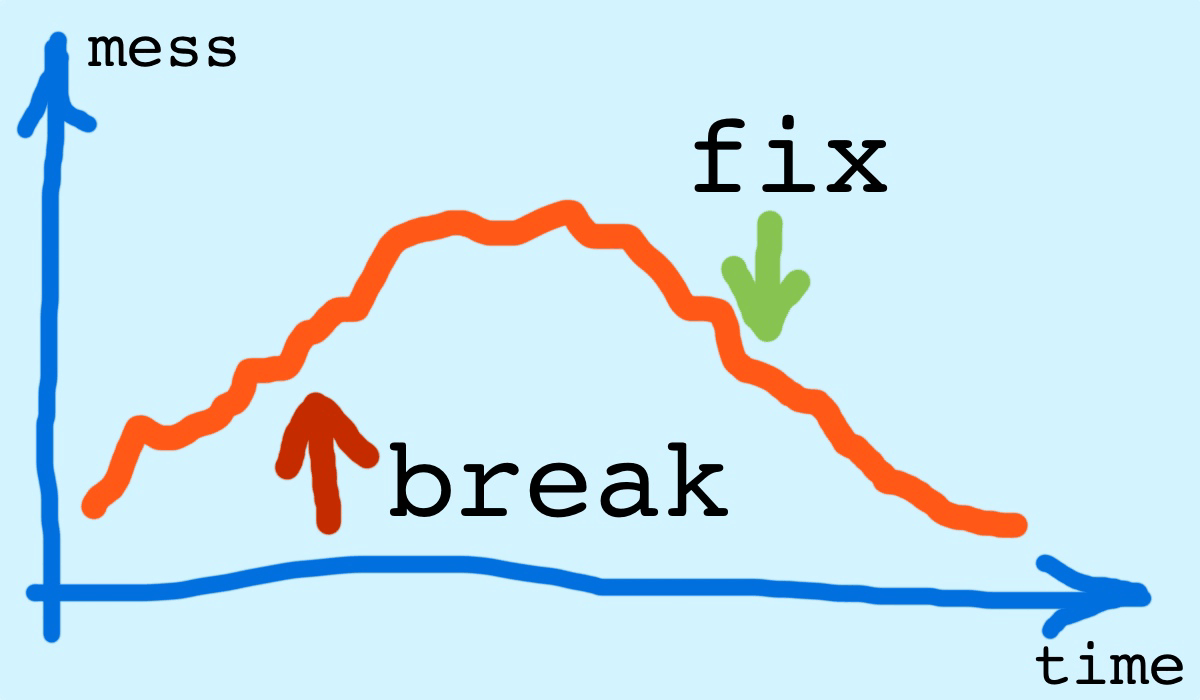
\includegraphics[width=.7\textwidth]{time-and-mess-diagram.png}\par
\lnSource{bugayenko2014blog0412}}

\lnPitch{
\pptBanner{\texttt{www.0pdd.com}}
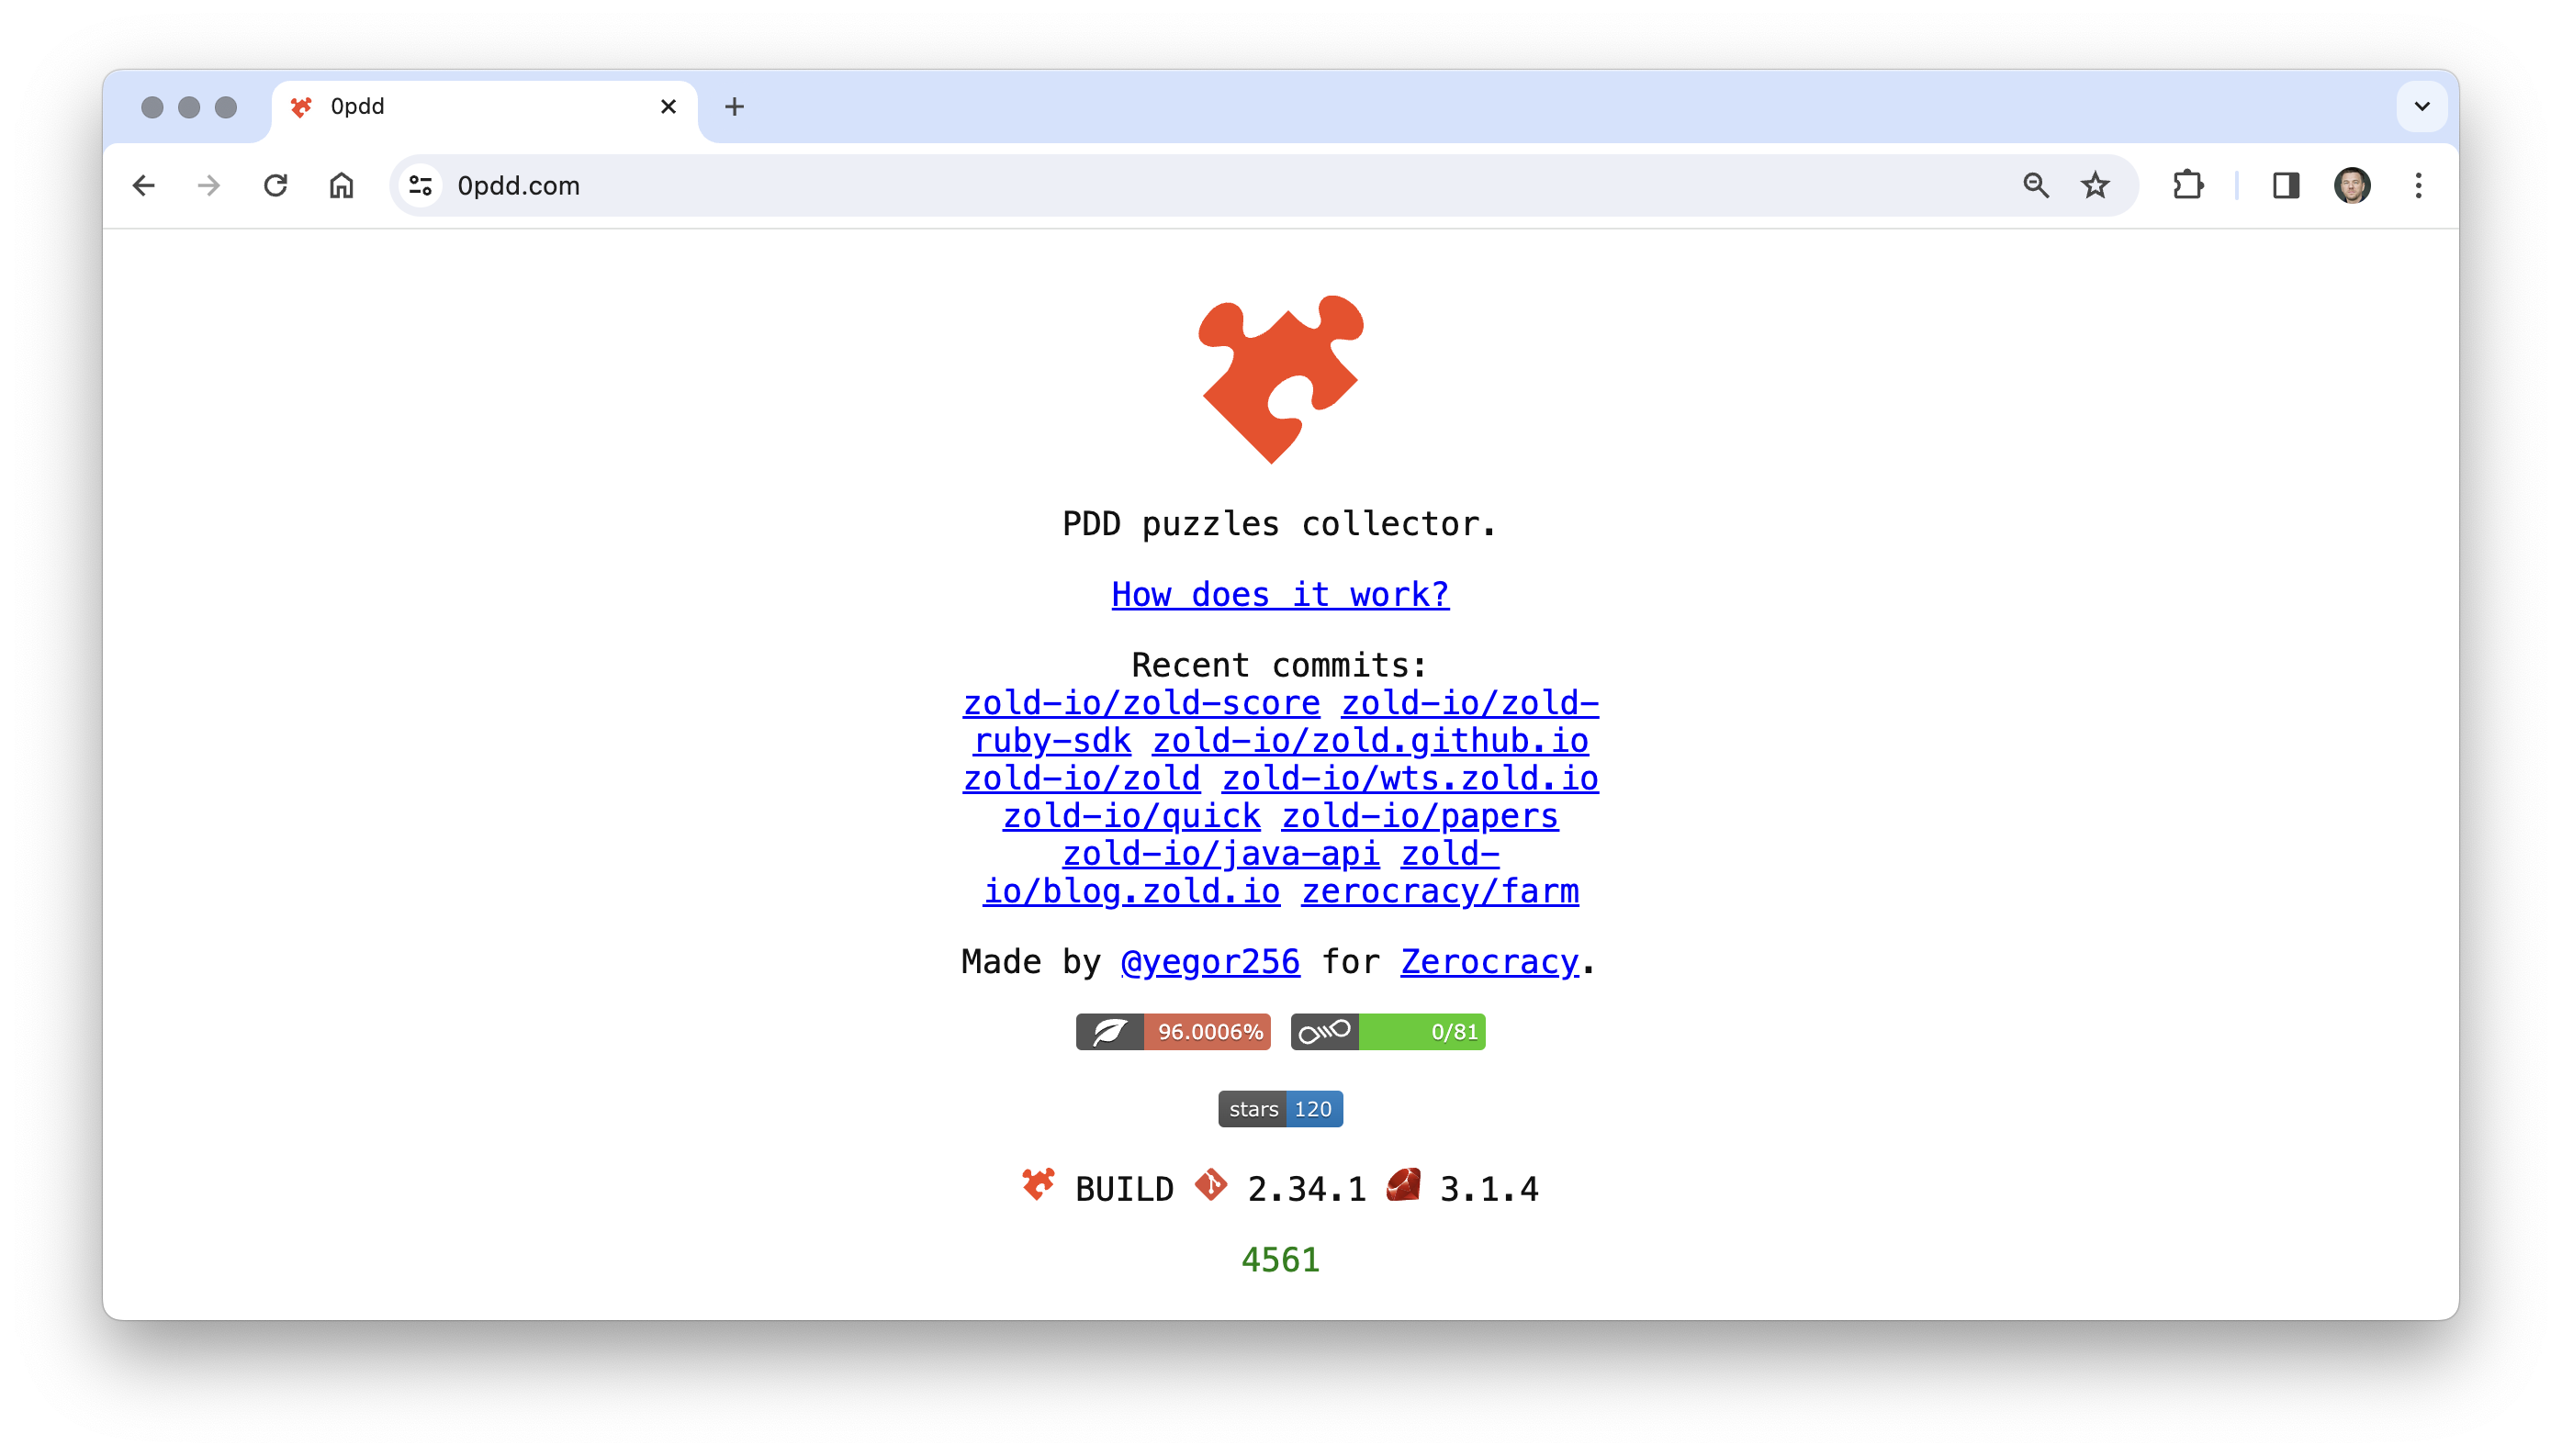
\includegraphics[width=.8\textwidth]{0pdd-front.png}}

\plush{\pptBanner{PDD Pipeline}
\begin{tikzpicture}[node distance=6em, every edge/.style={line width=.1em, draw, ->}, every node/.style={fill=white}]
\tikzstyle{actor} = [draw, line width=.1em,font={\Large},outer sep=.2em]
\node[actor] (coder1) {Coder \#1};
\node[actor,right=of coder1] (git) {Git};
\node[actor,right=of git] (0pdd) {0pdd.com};
\node[actor,below=of 0pdd] (tts) {TTS};
\node[actor,left=of tts] (coder2) {Coder \#2};
\path (coder1) edge node {push} (git);
\path (git) edge[bend left=30] node {webhook} (0pdd);
\path (0pdd) edge[bend left=30] node {submit ticket} (tts);
\path (coder2) edge[bend right=30] node {self-assign} (tts);
\path (coder2) edge[dashed] (git);
\end{tikzpicture}}

\lnPitch{
\pptBanner{250+ Puzzles in \texttt{objectionary/eo}}
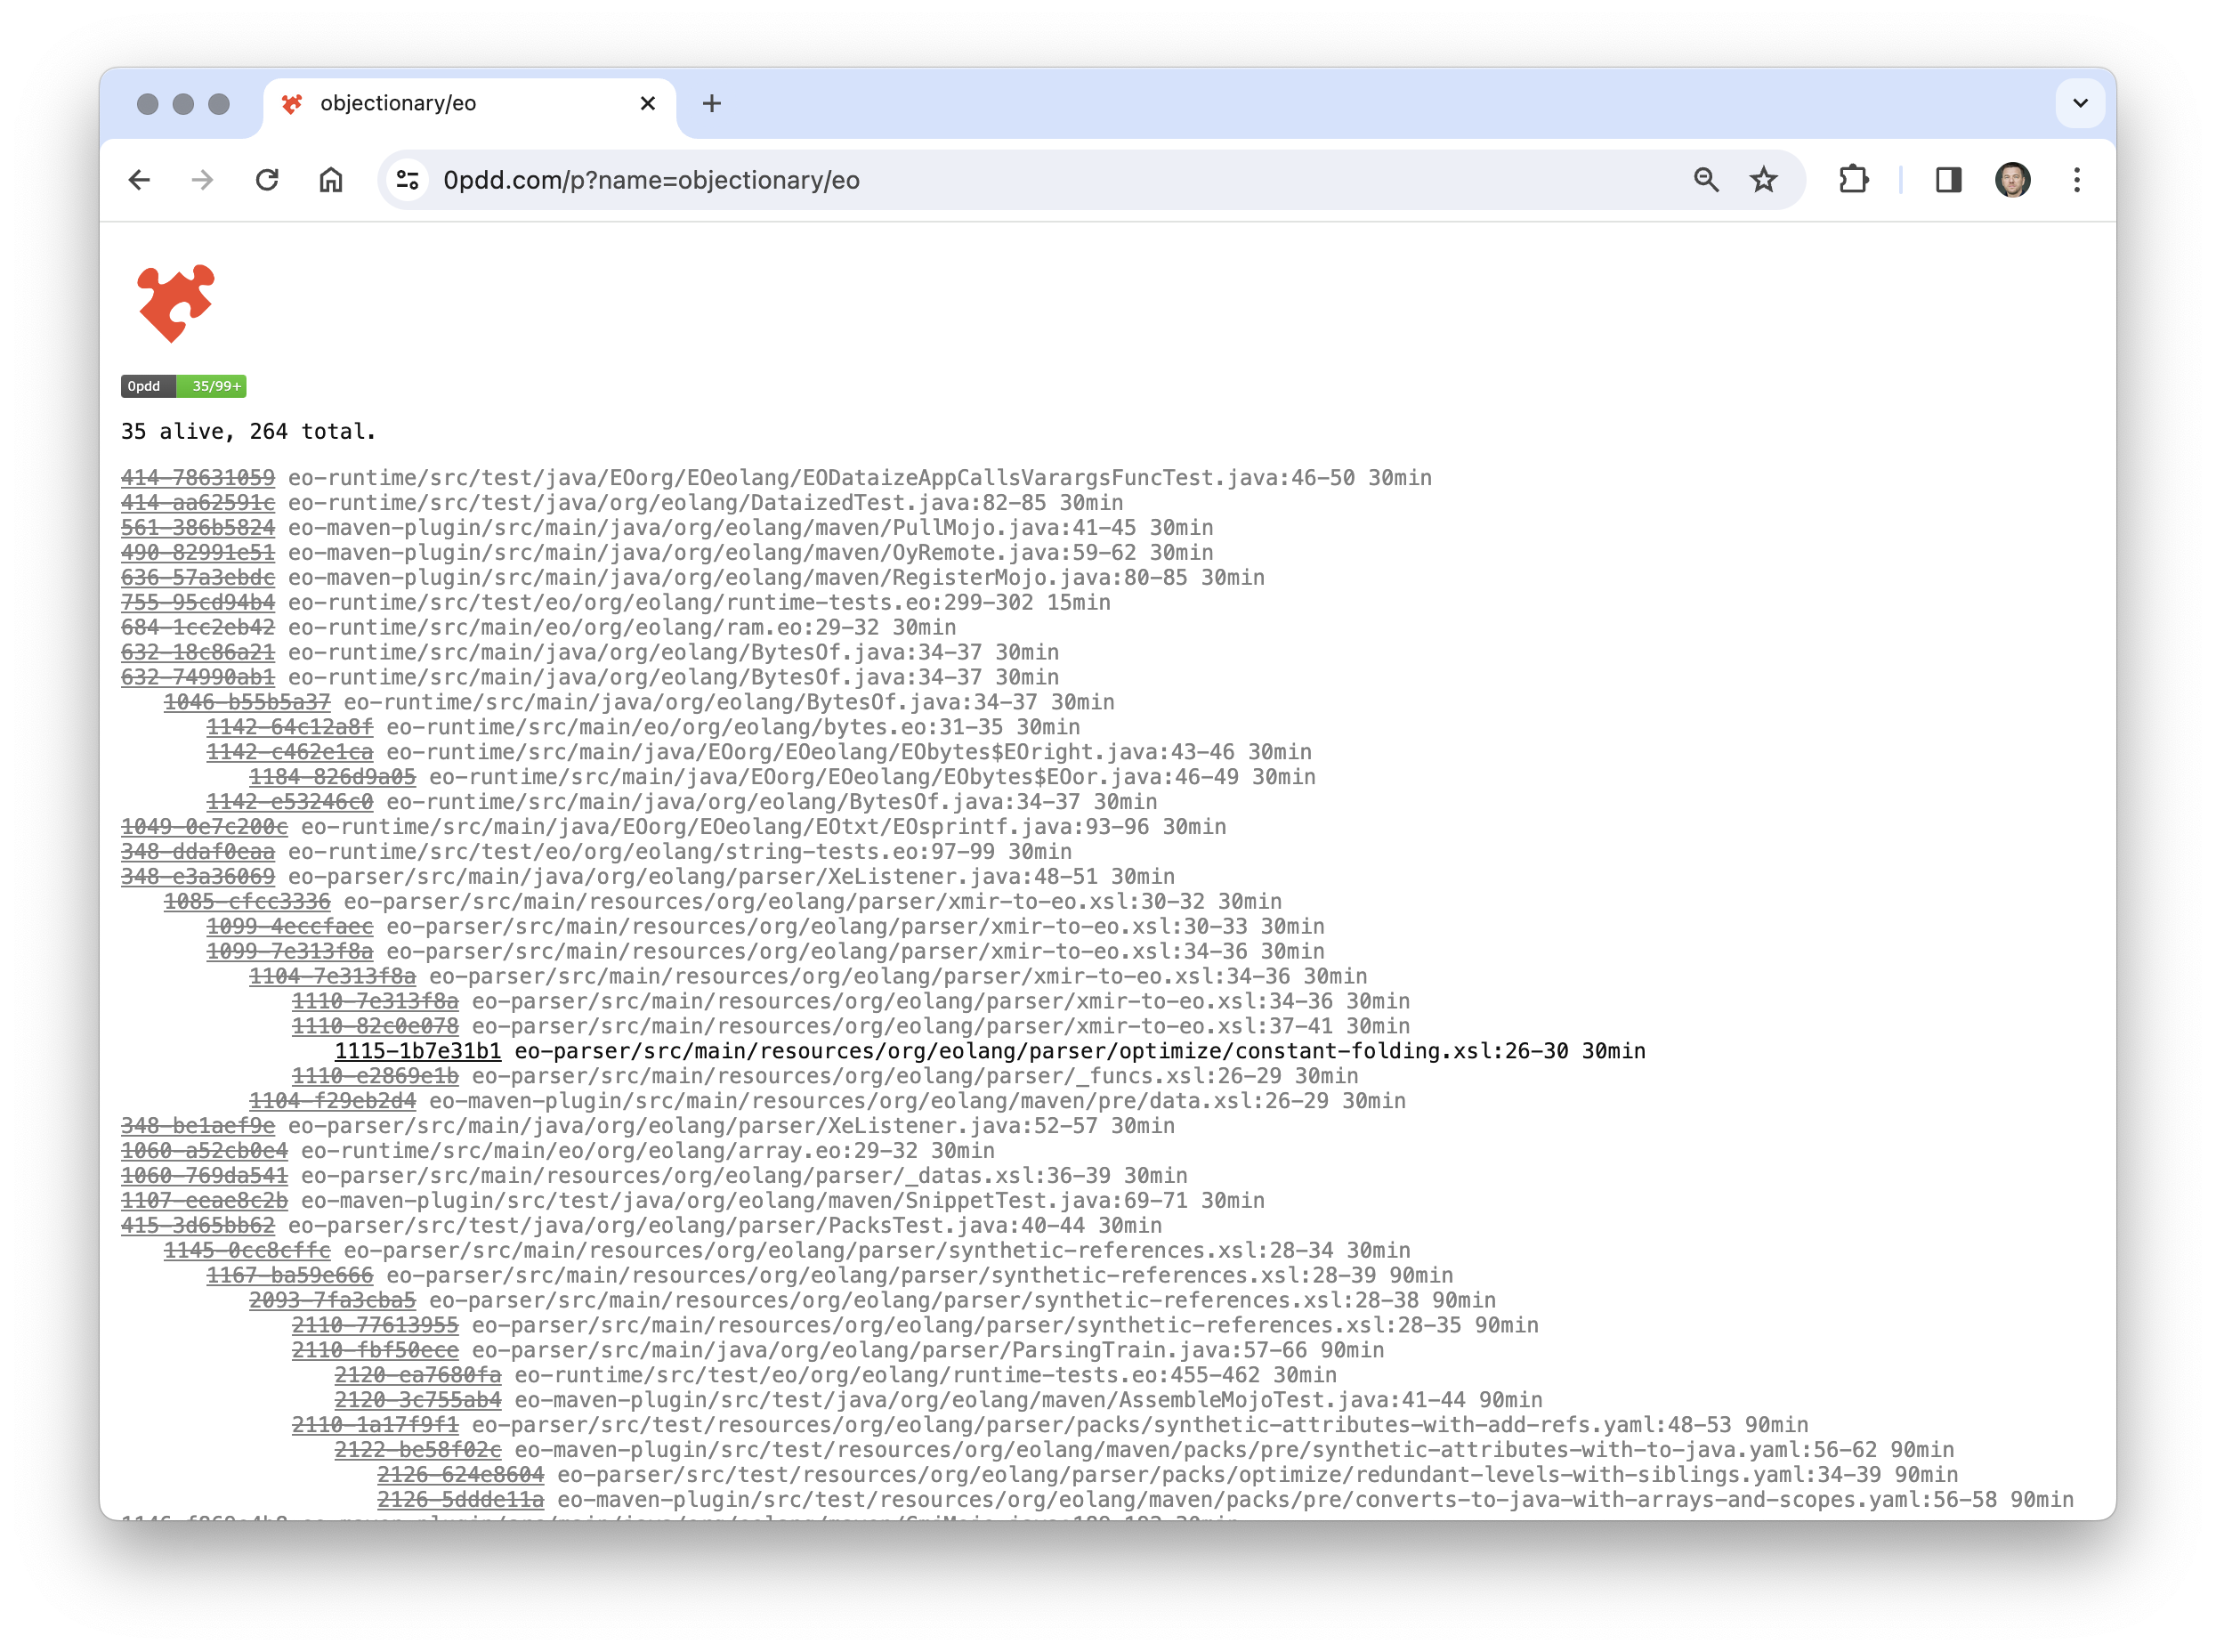
\includegraphics[width=.6\textwidth]{0pdd-screenshot.png}\par
{\small Source: \url{https://www.0pdd.com/p?name=objectionary/eo}\par}}

\lnPitch{
\pptBanner{Sample Ticket Submitted by 0pdd.com to \texttt{objectionary/eo}}
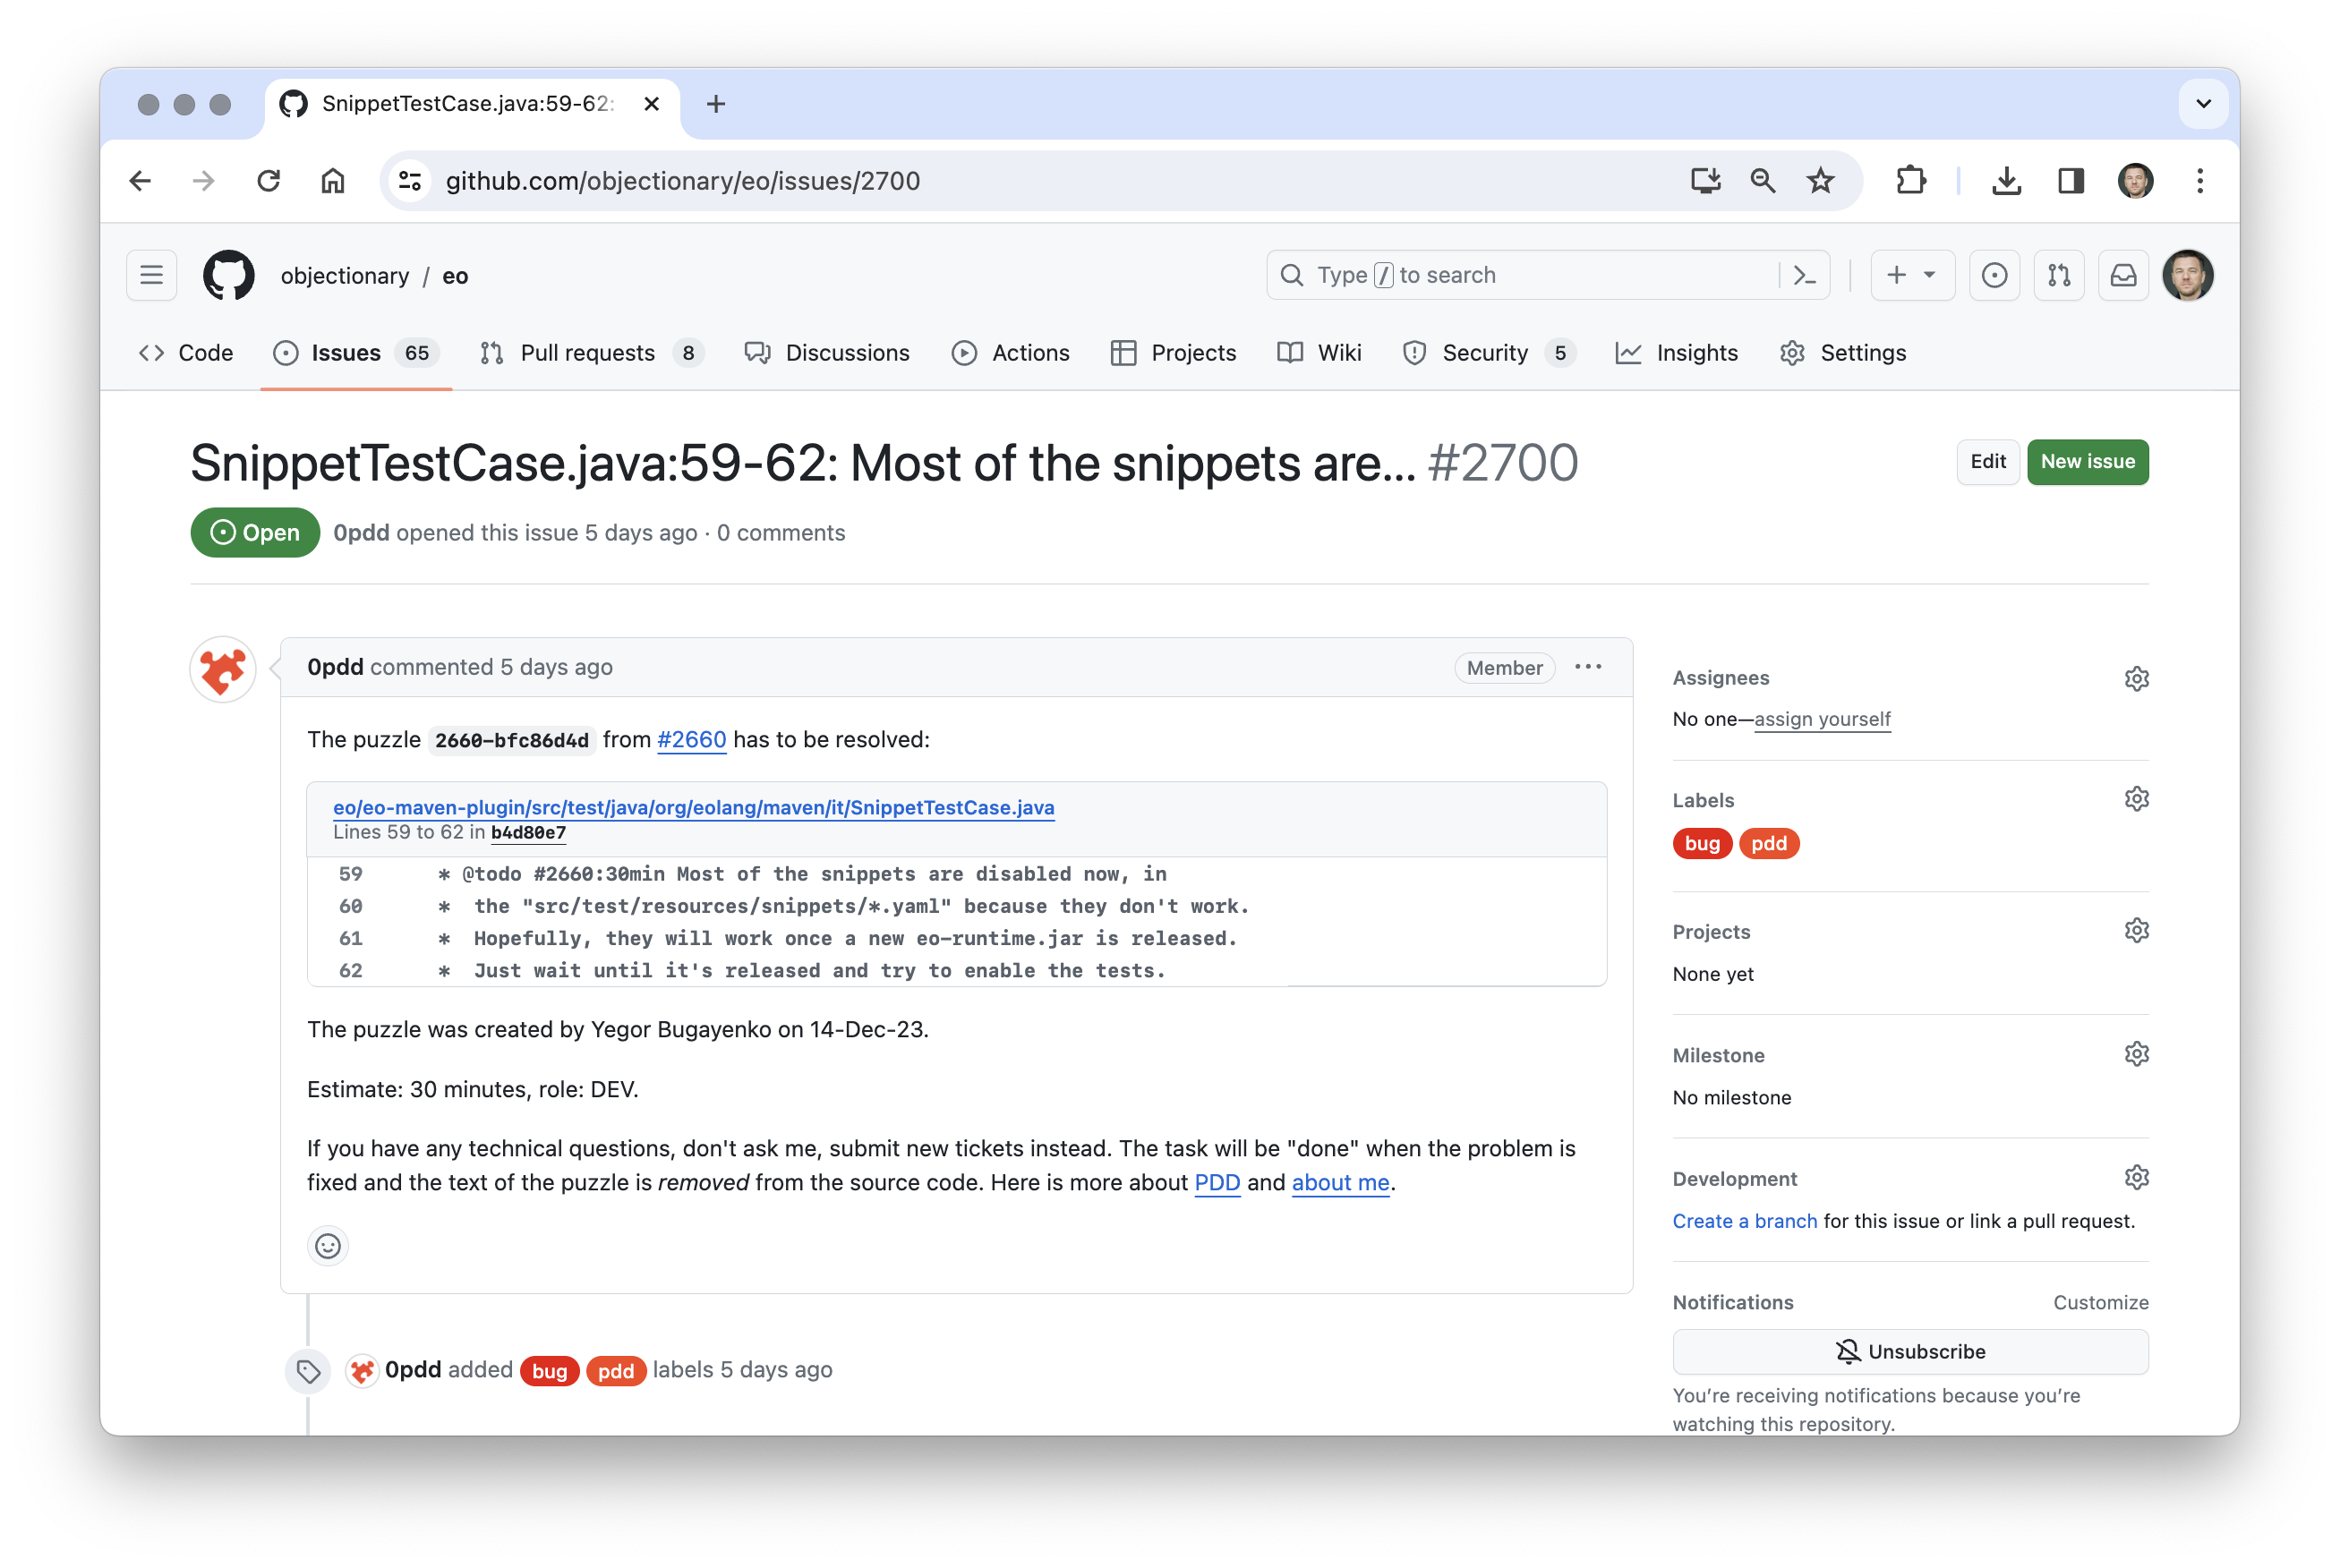
\includegraphics[width=.6\textwidth]{ticket.png}\par
{\small Source: \url{https://github.com/objectionary/eo/issues/2700}\par}}

\lnThought{Next, we AI to help us manage long backlog with puzzles}

\lnQuote
  [Giancarlo Succi]
  {giancarlo-succi}
  {This paper presents the benefits of considering the entire backlog when prioritizing tasks. We employ an iterative approach using Particle Swarm Optimization (PSO) to optimize a linear model with various preprocessing methods to determine the optimal model
for task prioritization within a backlog.}
  {bugayenko2023}

\end{document}
